%---------------------导言区---------------------------%
\documentclass[12pt,a4paper,UTF8]{ctexart}
	%10pt：正文字体为12pt，缺省为10pt；各层级字体大小会根据正文字体自动调整
	%a4paper：纸张大小a4；
	%UTF8：中文要求
\usepackage{geometry}%用于设置上下左右页边距
	\geometry{left=2.5cm,right=2.5cm,top=3.2cm,bottom=2.8cm}
\usepackage{xeCJK}
\usepackage{amsmath}
\usepackage{paralist}
\usepackage{enumerate}
\usepackage{booktabs}
\usepackage{multirow}
\usepackage{graphicx}
\usepackage{subfig}
\usepackage{setspace}
\usepackage{listings}
\usepackage{lastpage}
\usepackage{hyperref}
\usepackage{pdfpages}

%xeCJK：中文字体（如楷体，作者和机构需要用到）的设置
	%amsmath：数学公式
	%paralist，enumerate：自定义项目符号
	%booktabs：三线图，论文常用的表格风格
	%multirow：复杂表格
	%graphicx，float: 插入图片
	%subfig：并排排版图片、竖向排版图片
	%setspace：设置行间距等功能
	\setlength{\parindent}{2em}%正文首行缩进两个汉字
	%listings:用于排版各种代码；比如matlab的代码
	\lstset{language=Matlab}%matlab代码
	%lastpage:获取总页数;
	%hyperref:超链接,和lastpage搭配.
\usepackage{fancyhdr}
	%fancyhdr：一个很强大的宏包，用于自定义设计页面风格并命名以供调用。
	\pagestyle{fancy}
	\rhead{声光效应实验}
	\lhead{近代物理实验~~~实验报告}
	\cfoot{Page \thepage/\pageref{LastPage}}  %当前页\总页数
	\rfoot{\today}
		%分别是右页眉、左页眉、中页脚、右页脚
	\renewcommand{\headrulewidth}{0.4pt}
	\renewcommand{\theenumi}{(\arabic{enumi})}

%%%%%%%%%%%%%%%%%%%%%%%%%%%%%%%%%%%%%%%%%%%%%%%%%%%%%%%%%%
%%%%%%%%%%%%%%%%%%%%%%%%%正文开始%%%%%%%%%%%%%%%%%%%%%%%%%%
%%%%%%%%%%%%%%%%%%%%%%%%%%%%%%%%%%%%%%%%%%%%%%%%%%%%%%%%%%

\graphicspath{{声光效应示波器图片/}}
\begin{document}

%%begin-------------------标题与信息-----------------------%%

%%标题
\begin{center}
\LARGE\textbf{声光效应实验}
\end{center}

%%信息
\begin{doublespacing}
	%doublespacing：手动两倍行距
	\begin{tabular}{lr}
	 & \\
	 {实验人姓名：徐殊行~23343071} & {合作者姓名：王志超~23343062}\\
	 {实验时间：2025年4月11日} & {室温：30$^{\circ}$C~相对湿度：60\%}
	
	\end{tabular}
\end{doublespacing}

%%-------------------中英文摘要-----------------------%%
\begin{abstract}
	本实验通过研究超声波在介质中引发的声光效应，验证了Bragg衍射与Raman-Nath衍射的特性及差异。
	实验中利用半导体激光器、声光器件（铌酸锂晶体）及超声波信号源等装置，分别调节并观测两种衍射模式下的光强分布、偏转角度及频率调制现象。
	通过测量衍射效率、声速、中心频率和带宽等参数，证实了Bragg衍射的高效率特性（理论最大效率接近$100\%$）及其在声光调制中的优势，同时对比了Raman-Nath衍射的多级衍射特性。
	此外，通过声光模拟通信实验，演示了声光器件将电信号转换为光信号的过程，验证了其在光通信中的应用潜力。
	实验结果表明，声光效应可通过调节声波频率和功率实现光强、方向及频率的精确控制，为声光器件的设计与应用提供了实践依据。\cite{xujieping200x}\cite{li1989crystaloptics}\cite{huang200x}

	\noindent \textbf{关键词：声光效应；Bragg衍射；Raman-Nath衍射；衍射效率；声光调制} 
		
\end{abstract}
	
\renewcommand{\abstractname}{Abstract}

\begin{abstract}
	This experiment investigated the acousto-optic effect induced by ultrasonic waves in a medium, validating the characteristics and distinctions between Bragg diffraction and Raman-Nath diffraction.
	Utilizing semiconductor lasers, an acousto-optic device (lithium niobate crystal), and an ultrasonic signal generator, the intensity distribution, deflection angles, and frequency modulation of light under both diffraction modes were observed and analyzed.
	By measuring parameters such as diffraction efficiency, sound velocity, central frequency, and bandwidth, the high efficiency of Bragg diffraction (with a theoretical maximum efficiency approaching $100\%$) and its advantages in acousto-optic modulation were confirmed, while the multi-level diffraction properties of Raman-Nath diffraction were comparatively demonstrated.
	Additionally, an acousto-optic analog communication experiment illustrated the process of converting electrical signals into optical signals using the device, validating its potential applications in optical communication.
	The results indicate that the acousto-optic effect enables precise control of light intensity, direction, and frequency by adjusting ultrasonic frequency and power, providing practical insights for the design and application of acousto-optic devices.

	\noindent \textbf{Keywords: acousto-optic effect~~ Bragg diffraction~~ Raman-Nath diffraction~~ diffraction efficiency~~ acousto-optic modulation}
\end{abstract}

%%-------------------正文部分-----------------------%%

\subsection*{【实验目的】}

\begin{enumerate}[(1)]
	\item 理解声光效应的原理，了解 Raman-Nath 衍射和 Bragg 衍射的分别。
	\item 测量声光器件的衍射效率、中心频率和带宽等参数。
	\item 声光模拟通信实验。
\end{enumerate}

\subsection*{【实验原理】}

\subsubsection*{1.声光效应的物理本质——光弹效应}
	声光效应的物理本质源于光弹效应，即介质在声场作用下因应力产生应变，导致其光学性质的周期性调制。
	根据介质介电张量的逆张量变化关系，折射率椭球方程的系数可表示为：

	\begin{equation}
		\eta_{ij}x_{i}x_{j}  = 1
	\end{equation}
	其中$\eta_{ij}$是介质介电张量的逆张量，是一个二阶对称张量。
	介质中存在声场，介质内部就受到应力而发生声应变，从而引起介质光学性质的变化。
	这种变化反映在介质光折射率的或折射率椭球方程系数的变化上。在一级近似下，$\Delta \eta_{ij}$与应变$\S_{kl}$成线性关系：

	\begin{equation}
		\Delta \eta_{ij} = P_{ijkl}S_{kl}
	\end{equation}
	
	其中$P_{ijkl}$是光弹系数，是一个四阶张量，表征了应变对介质光学性质的影响程度。
	为简单起见，这里只考虑各向同性介质中声纵波的情况，这样折射率 n 和光弹系数 P 都可以看作常量。
	如此，上式可以简化为：

	\begin{equation}
		\Delta \left( \frac{1}{n^2} \right) = PS 
	\end{equation}

	其中，\( P \) 为光弹系数，\( S = S_0 \sin(kx - \Omega t) \) 为声应变波（\( k = \Omega / v_s \)，\( \Omega = 2\pi f \)，\( v_s \) 为声速）。
	由此推导出折射率的周期性变化：
	
	\begin{equation}
		\Delta n = \frac{1}{2} n^3 P S_0 \sin(kx - \Omega t) = \mu \sin(kx - \Omega t)
	\end{equation}

	于是，介质中折射率分布为：

	\begin{equation}
		n(x,t) = n_0 + \mu \sin(kx - \Omega t)
	\end{equation}
	
	其中，$\mu = \frac{1}{2} n^3 P S_0$，是“声致折射率变化“的最大值。

	压电换能器将驱动电信号 U(t)转换为声信号，入射平面波与声波在介质中相遇，当光通过线度为 l 的声光互作用介质时，其位相改变为
	
	\begin{equation}
		\phi(x) = \phi_0 +  \mu k_0 \sin(kx - \Omega t)
	\end{equation}
	
	其中 $k_0$＝$2\pi／\lambda_0$ 为真空中光波数，$\lambda_0$ 是真空中的光波长，$\Delta\phi_0$＝$nk_0l$ 为光通过不存在超声波的介质后的位相滞后，项 $\mu k_0\sin(kx－\Omega t)$为由于介质中存在超声波而引起的光的附加位相延迟。
	它在ｘ方向周期性地变化，犹如光栅一般，故称"位相光栅"。
	这就使得光波阵面由原先的平面变为周期性的"位相绉折"，这就改变了光的传播方向，也就是产生了所谓的衍射。
	与此同时，光强分布在时间和空间上又作了重新分配，也就是衍射光强受到了声调制。
		
	\begin{figure}[h!]
		\centering
		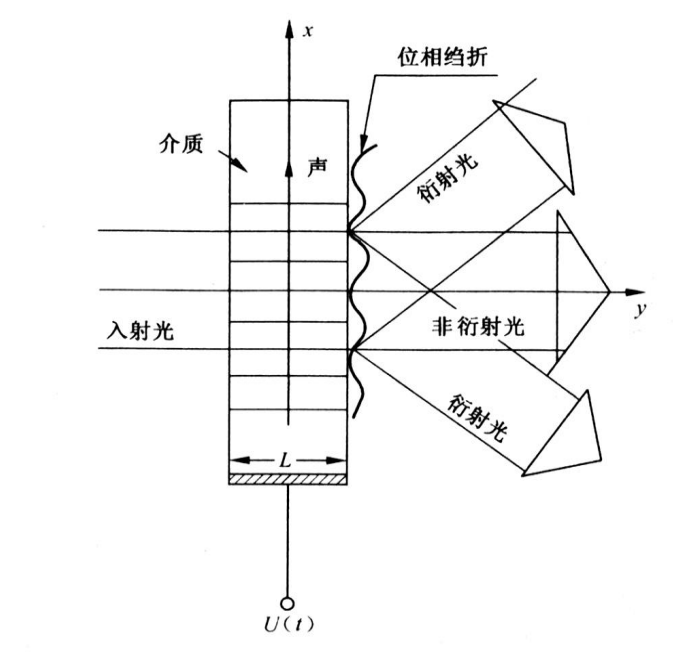
\includegraphics[width=0.7\linewidth]{原理图.png}
		\caption{声光效应原理示意图}
		\label{fig:acousto_optic_principle}
	\end{figure}	
	
	这种调制形成“声光栅”，光通过时因相位延迟而发生衍射。根据声光作用长度 \( L \) 与声波长 \( \Lambda \) 的关系，衍射分为两类：

	\begin{enumerate}
		\item \textbf{Raman-Nath衍射}：当 \( \lambda L / \Lambda^2 \ll 1 \) 时，光近似垂直于声波面入射，声光介质等效为平面相位光栅，产生多级对称衍射（如 ±1、±2 级），其衍射效率由贝塞尔函数描述：
		\begin{equation}
		\eta^{(m)} = J_m^2 \left( 2\zeta L \sin c \left[ \frac{K L}{2 \cos \theta_i} \left( \sin \theta_i + m \frac{K}{k} \right) \right] \right)
		\end{equation}
		
		\item \textbf{Bragg衍射}：当 \( \lambda L / \Lambda^2 \gg 1 \) 时，光以 Bragg 角 \( \theta_B = \arcsin(\lambda / 2\Lambda) \) 斜入射，声光介质表现为体光栅，仅存在 0 级和 1 级衍射。其衍射效率为：
		\begin{equation}
		\eta_B = \sin^2 \left( \frac{\pi}{\sqrt{2\lambda_0 \cos \theta_i}} \sqrt{M_2 P_a \frac{L}{H}} \right)
		\end{equation}

	\end{enumerate}
	
\subsubsection*{2.衍射效率}\cite{xujieping200x}
	
	\paragraph{Raman-Nath衍射}
	当声光作用长度较短（$\lambda L / \Lambda^2 \ll 1$）时，形成多级衍射，效率由贝塞尔函数描述。
	\begin{equation}
		\eta_R^{(m)} = J_m^2 \left( 2\zeta L \cdot \mathrm{sinc} \left[ \frac{K L}{2 \cos \theta_i} \left( \sin \theta_i + m \frac{K}{k} \right) \right] \right) 
		\label{eq:raman-eff}
	\end{equation}

	\paragraph{Bragg衍射}
	当声光作用长度较长（$\lambda L / \Lambda^2 \gg 1$）时，仅存在0级和1级衍射，效率由正弦平方函数描述。
	\begin{equation}
		\eta_B = \sin^2 \left[ \frac{\pi}{\sqrt{2\lambda_0 \cos \theta_i}} \sqrt{M_2 P_a \frac{L}{H}} \right]
		\label{eq:bragg-eff}
	\end{equation}

\subsection*{【实验仪器】}
	\begin{table}[h!]
		\centering
		\begin{tabular}{|p{4cm} p{4cm} p{6cm}|}
			\hline
			仪器名称 & 型号 & 参数 \\
			\hline\hline
			激光器 & 南京浪博科教仪器 & - \\
			
			行波声光器件 & 南京浪博科教仪器 & $f_{0}$ = 100 MHz \\
			
			CCD光强分布测量仪 & LM601S & 2700位光敏元 \\
			
			频率计 & GFC-8131 & - \\
			
			声光效应功率信号源 & SO-2000 & - \\
			
			示波器 & TBS~2000~SERIES & $100Mhz~~1 GS/s$ \\
			\hline		
		\end{tabular}
		\caption{实验仪器及参数}
		\label{tab:instruments}
	\end{table}

\subsection*{【实验内容】}
	在实验开始前认真阅读声光效应仪的说明书，正确连接各个部件，准直光路。
	相应的光路图如图\ref{fig:acousto_optic_principle}所示。

	\begin{figure}[h!]
		\centering
		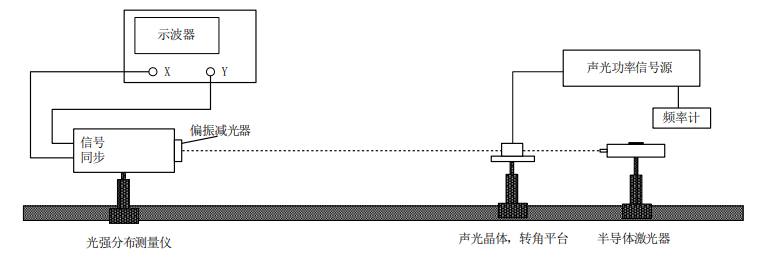
\includegraphics[width=0.7\linewidth]{光路图.png}
		\caption{声光效应光路图}
		\label{fig:acousto_optic_principle}
	\end{figure}

	\begin{itemize}
		\item 根据教材描述，分别调出 Raman-Nath 衍射和 Bragg 衍射，初步对比两种衍射的条件和特点。
		
		\item 对示波器定标：用示波器测量衍射角，先要解决“定标”的问题。即示波器 X 方向上的 1 格等于 CCD 器件上多少象元，从而对应 CCD 上 X 方向上的多少距离。
		
		\item 在 Bragg 衍射条件下，固定超声波功率，改变超声波的频率 \( f_s \)，记录 1 级（面向接收屏，左侧第一衍射级为 1 级，右侧第一衍射级为 -1 级）衍射光最强时，1 级衍射光相对于 0 级透射光的偏转角 \(\phi\)。测出 10 组 \( (\phi, f_s) \) 值，并计算声速 \( v_s \)。同时定出声光器件中心频率（1 级衍射光最强时对应的频率）和带宽（衍射光强从极大值的两边下降到 \( 1/\sqrt{2} \) 对应的频带宽度）。注意计算声速中，Bragg 角 \( \theta_B \) 是指介质内的角度，而直接测出的角度 \( \phi \) 是空气中的角度，应根据折射定律进行换算。其中声光晶体二氧化碲的折射率 \( n = 2.26 \)，半导体激光器波长 \( \lambda = 650\,\text{nm} \)。
		
		\item 将超声波频率固定在步骤 4 中获得的中心频率上，并调节晶体角度使其满足 Bragg 衍射条件，测量衍射光强度与超声波电流的关系曲线。测定 Bragg 衍射下的最大衍射效率 \( I_1/I_{\text{总}} \)。其中 \( I_{\text{总}} \) 为未发生声光衍射时的 0 级光的强度（\( I_{\text{总}} \) 也可取为衍射后的 0 级和 1 级光的光强之和），\( I_1 \) 为 1 级衍射光的强度。
		
		\item 在 Raman-Nath 衍射下（光束垂直入射，调节 +1 级与 -1 级衍射强度相等），将电流调制最大值，分别测量：
		
		\begin{itemize}
			\item 测量 \( \pm 1 \) 级衍射光的效率与频率的依赖关系；
			\item \( \pm 1 \) 级衍射角 \( \theta_m \) 与频率的依赖关系（\( \pm 1 \) 级衍射光相对于 0 级在晶体中的偏转角）。
		\end{itemize}

		每组实验要测量 10 点以上（效率为 \( I_n/I_{\text{总}} \)，\( n \) 指特定衍射级，\( I_{\text{总}} \) 为总光强）。
		
		\item 在步骤 6 中，选取衍射效率最高时所对应的频率，测量 \( \pm 1 \) 级衍射光的衍射效率与电流的依赖关系，并与 Bragg 衍射下的衍射效率进行比较。实验要测量 10 点以上。
		
		\item 在 Raman-Nath 衍射下，选取衍射效率最高时所对应的频率，将电流调到最大值，记录偏离垂直入射时 \( \pm 1 \) 和 \( \pm 2 \) 级衍射光的衍射效率以及相应的偏离角度（选择 1-2 个旋转角度，偏离角度可通过晶体旋转台测得）。
		
		\item 进行声光模拟通信实验。分别观测接收 0 级和 1 级衍射光信号时，示波器上的波形，并与发射器的波形进行对比，判断其同相还是反相。改变超声波功率，注意观察模拟通信接收器的音乐的变化，分析原因。
		
		\item 实验完成后请将实验设备的各个元件收拾好，并整理好桌椅。
	\end{itemize}

\subsection*{【实验过程和数据处分析处理】}
	仔细阅读上述实验过程，并检查实验仪器完整可用之后我们开始实验。

\subsubsection*{1.光路调整}
	按照实验要求，我们首先调整光路。

	\begin{itemize}
		\item 首先在不给声光晶体加电的情况下，调整光路，使得激光器发出的激光能够通过声光晶体。
		\item 此时调整CCD的位置，使得激光器发出的激光能够打在CCD的中心。
		\item 然后将激光器功率调至较大时，给声光晶体加电，用光屏承接衍射光，使得光屏上出现清晰的衍射斑。
		\item 此时轻微转动声光晶体的角度，能够观察到衍射光斑的强度随着角度变化，利用肉眼可判断出此时发生的是Bragg衍射还是Raman-Nath衍射。
		\item 随后可以撤去光屏，直接用CCD接收衍射光，并在示波器上观察衍射光斑的强度。
	\end{itemize}

	调整完成之后观察示波器上的图像，如图\ref{fig:oscilloscope_images}所示，确实能够观察到Raman-Nath衍射（左）和Bragg衍射（右）的图像。

	\begin{figure}[h!]
		\centering
		\begin{minipage}[t]{0.48\textwidth}
			\centering
			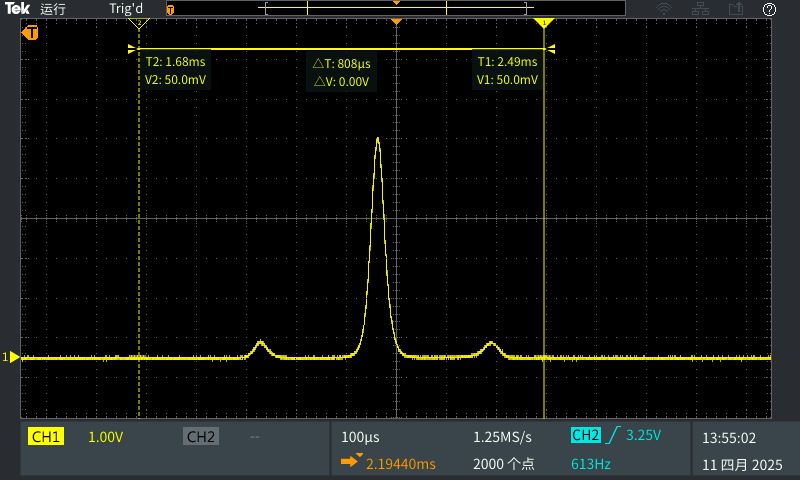
\includegraphics[width=\linewidth]{TEK00002.PNG}
		\end{minipage}
		\hfill
		\begin{minipage}[t]{0.48\textwidth}
			\centering
			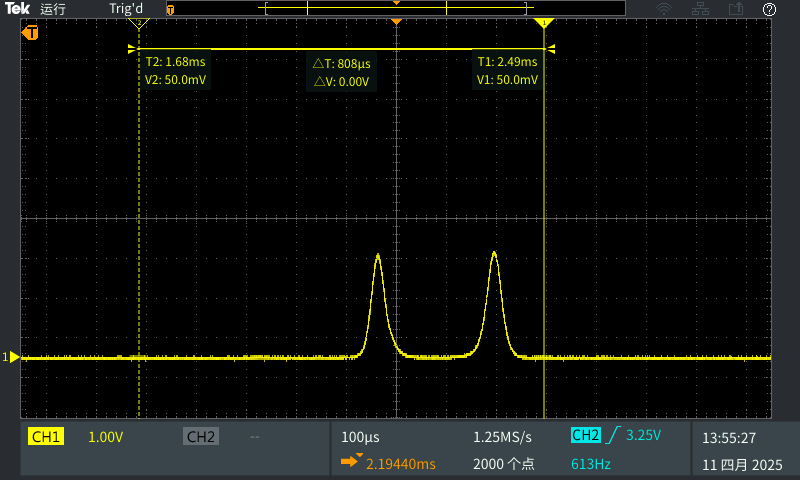
\includegraphics[width=\linewidth]{TEK00003.PNG}
		\end{minipage}
		\caption{两种衍射对应的示波器图像}
		\label{fig:oscilloscope_images}
	\end{figure}
	
\subsubsection*{2.对示波器定标} 
	为了能够从示波器上的图像中直接获得衍射光的衍射角，我们需要对示波器进行定标。
	CCD的参数上读出其总长度和每一个光敏单元的大小。
	然后利用示波器的测量功能读出整个CCD长度在示波器上对应的 $\Delta T $。
	最后使用刻度尺测量从声光晶体到CCD的距离。

	定标过程中示波器的图像如图\ref{fig:calibration_measurement}所示：
	
	\begin{figure}[h!]
		\centering
		\begin{minipage}[t]{0.48\textwidth}
			\centering
			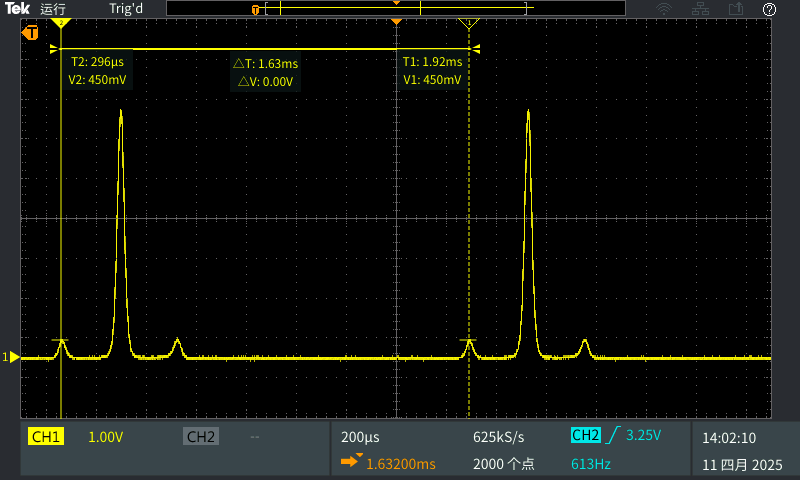
\includegraphics[width=\linewidth]{TEK00006.PNG}
		\end{minipage}
		\hfill
		\begin{minipage}[t]{0.48\textwidth}
			\centering
			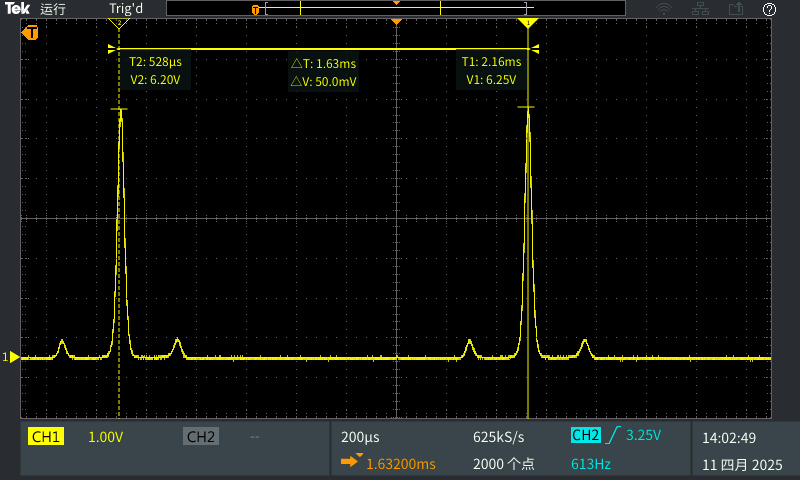
\includegraphics[width=\linewidth]{TEK00007.PNG}
		\end{minipage}
		\caption{示波器定标过程}
		\label{fig:calibration_measurement}

	\end{figure}

	测量得到的参数如下表所示

	\begin{table}[h!]
		\centering
		\begin{tabular}{|c|c|c|}
			\hline
			\textbf{参数} & \textbf{符号} & \textbf{数值} \\
			\hline
			CCD总长度 & $ L $ & 29.7 $\mathrm{mm}$ \\
			\hline
			每个光敏单元大小 & $d$ & 11 $\mu \mathrm{m}$ \\
			\hline
			示波器上一个周期的宽度 & $T$ & 1.63 ms \\
			\hline
			声光晶体到CCD的距离 & $D$ & 329 mm \\
			\hline
		\end{tabular}
		\caption{示波器定标参数}
		\label{tab:oscilloscope_calibration}
	\end{table}
	
	根据上述参数，我们可以计算出示波器上的时间与衍射角度的换算关系：
	记$\Delta T$ 是示波器上测得的横向距离，实际衍射光之间的距离为$ x $，对应的偏转角为$\phi$ 

	\begin{align}
		x & = \frac{\Delta T}{T} L \\
		\phi & = \mathrm{arctan}\left(\frac{x}{D}\right)
	\end{align}

	这样我们可以用公式将示波器上的距离换算成衍射光的偏转角度，便于后续测量。

\subsubsection*{3.Bragg衍射条件下超声频率与衍射角之间的关系}
	在正式测量开始之前我们先大致调节了超声频率的范围，发现在$ 80~-~100\mathrm{Hz} $ 范围内实验现象较为明显。
	在测量超声频率和衍射角之间的关系时，我们便采用上述的频率范围。	

	按照上述方法，我们测量得到了以下表\ref{tab:frequency_diffraction}中的数据
	\begin{table}[h!]
		\centering
		\begin{tabular}{|c|c|c|c|}
			\hline
			\textbf{超声频率 $f_s$ (MHz)} & \textbf{示波器测量值 $\Delta T$ ($\mu$s)} & \textbf{空气中偏转角 $\phi$ (°)} & \textbf{晶体中偏转角 (°)} \\
			\hline
			80.408 & 223 & 0.0123 & 0.0279 \\
			\hline
			82.074 & 227 & 0.0126 & 0.0284 \\
			\hline
			84.045 & 232 & 0.0128 & 0.0290 \\
			\hline
			86.025 & 238 & 0.0132 & 0.0298 \\
			\hline
			88.008 & 244 & 0.0135 & 0.0305 \\
			\hline
			90.043 & 248 & 0.0137 & 0.0310 \\
			\hline
			92.095 & 252 & 0.0140 & 0.0315 \\
			\hline
			94.043 & 256 & 0.0142 & 0.0320 \\
			\hline
			96.028 & 262 & 0.0145 & 0.0328 \\
			\hline
			98.034 & 268 & 0.0148 & 0.0335 \\
			\hline
			100.01 & 272 & 0.0151 & 0.0340 \\
			\hline
		\end{tabular}
		\caption{一级衍射光偏转角随超声频率的变化关系}
		\label{tab:frequency_diffraction}
	\end{table}

	相应地，我们得到了图\ref{fig:frequency_angle}，可见二者基本成线性关系，我们可以通过线性拟合的方式来得到晶体中的声速。
	
	\begin{figure}[h!]
	    \centering
	    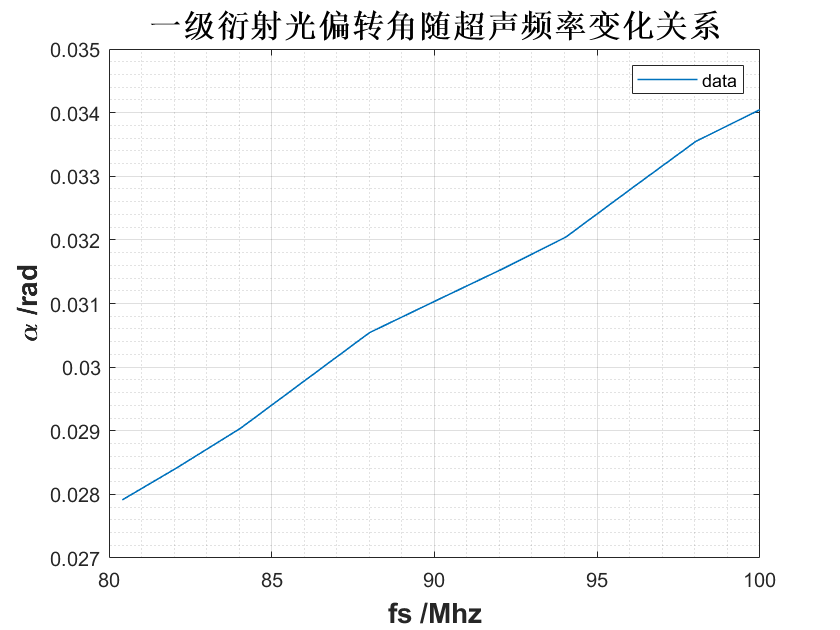
\includegraphics[width=0.8\textwidth]{偏转角随超声频率.png}
	    \caption{一级衍射光偏转角随超声频率的变化关系}
	    \label{fig:frequency_angle}
	\end{figure}

	对二者进行线性拟合，可以得到实验上测得的晶体中的声速为$ 922.22 \mathrm{m/s}$ 。
	这一结果的可靠性较高\cite{xujieping200x}，主要体现在以下几个方面：首先，从图\ref{fig:frequency_angle}可以看出，
	实验数据点基本呈现良好的线性关系，说明测量过程中系统误差较小；
	其次，我们采用了多个频率点进行测量，增加了数据的统计可靠性；
	最后，测量过程中示波器显示的波形较为稳定，减小了读数误差。
	不过，由于示波器上波形存在微小抖动，可能会对最终结果产生一定影响。

	而为了测量晶体的中心频率和带宽，我们再次改变频率进行测量，这次需要记录衍射效率和超声频率之间的关系，如表\ref{tab:bragg_efficiency}所示

	\begin{table}[h!]
		\centering
		\begin{tabular}{|c|c|c|}
			\hline
			\textbf{$f_s$ (MHz)} & \textbf{$I_0$ (V)} & \textbf{$I_1$ (V)} \\
			\hline
			80.01 & 0.33 & 0.43 \\
			\hline
			84.03 & 0.29 & 0.45 \\
			\hline
			88.00 & 0.27 & 0.47 \\
			\hline
			91.99 & 0.22 & 0.45 \\
			\hline
			96.00 & 0.27 & 0.45 \\
			\hline
			100.01 & 0.27 & 0.44 \\
			\hline
			104.00 & 0.31 & 0.42 \\
			\hline
			108.00 & 0.32 & 0.39 \\
			\hline
			112.90 & 0.35 & 0.36 \\
			\hline
			116.01 & 0.39 & 0.35 \\
			\hline
			120.00 & 0.45 & 0.31 \\
			\hline
		\end{tabular}
		\caption{Bragg衍射效率与频率的关系}
		\label{tab:bragg_efficiency}
	\end{table}

	我们即可得出此样品的中心频率为$ 90 \mathrm{MHz}$ 左右，带宽为$ 4.043 \mathrm{MHz}$ 。
		
\subsubsection*{4.Bragg衍射光强和超声波电流的关系}
	我们将超声波频率固定在上述测得的中心频率上，调节晶体角度，能够观察到布拉格衍射。
	此时测量衍射光强度和超声波电流的关系曲线。

	首先我们测量得到总光强为$I_{总} = 6.7 \mathrm{V} $ 
	绘制出衍射光强随超声波电流的变化关系曲线如图\ref{fig:diffraction_intensity}所示

	\begin{figure}[h!]
		\centering
		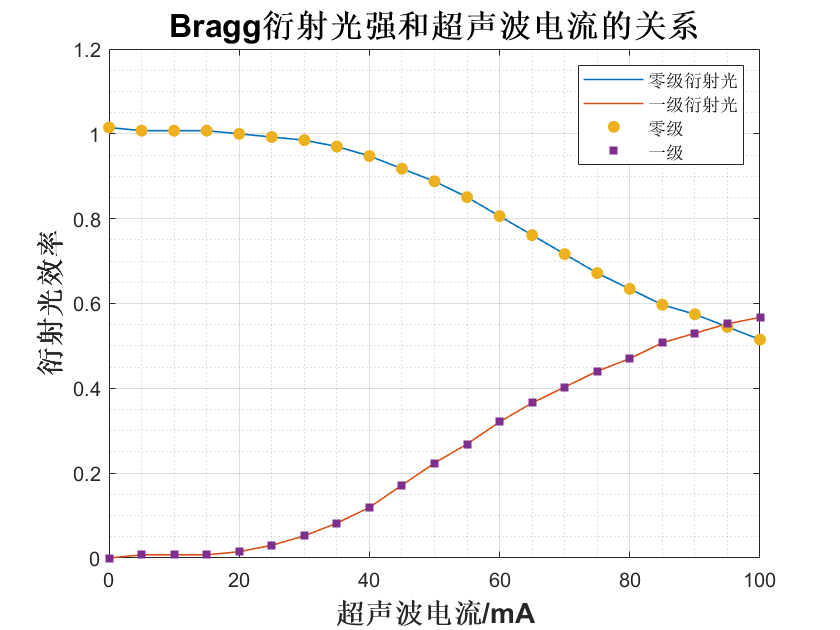
\includegraphics[width=0.8\textwidth]{衍射光强随超声波电流.PNG}
		\caption{衍射光强随超声波电流的变化关系}
		\label{fig:diffraction_intensity}
	\end{figure}

	可见，一级衍射光强度随超声波电流的增大而增大，同时零级衍射光光强有所下降。
	但是在电流达到$ 80 \mathrm{mA} $ 之后，一级衍射光强度基本不再增大。
	
\subsubsection*{5.Raman-Nath衍射光强和超声波电流的关系}
	我们先调节晶体的角度，能够在示波器上观察到Raman-Nath衍射，将超声电流调节至最大值，再稍作调节，使得正负一级衍射光的强度基本相等。
	从图\ref{fig:raman_nath_diffraction}中可以看出此时已调节出Raman-Nath衍射，并且利用示波器的测量功能，可以确认正负一级衍射光的强度基本相等，符合实验的要求。

	\begin{figure}[h!]
		\centering
		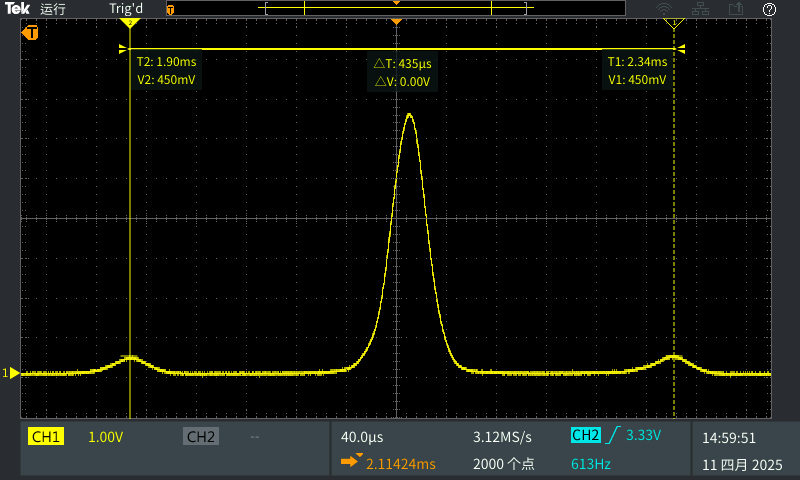
\includegraphics[width=0.8\textwidth]{TEK00017.PNG}
		\caption{Raman-Nath衍射，正负一级衍射强度相等}
		\label{fig:raman_nath_diffraction}
	\end{figure}

	首先测量正负一级的衍射光效率和超声波频率的依赖关系，结果如图\ref{fig:rn_efficiency_frequency}和图\ref{fig:rn_angle_frequency}所示。

	\begin{figure}[h!]
		\centering
		\begin{minipage}{0.48\textwidth}
			\centering
			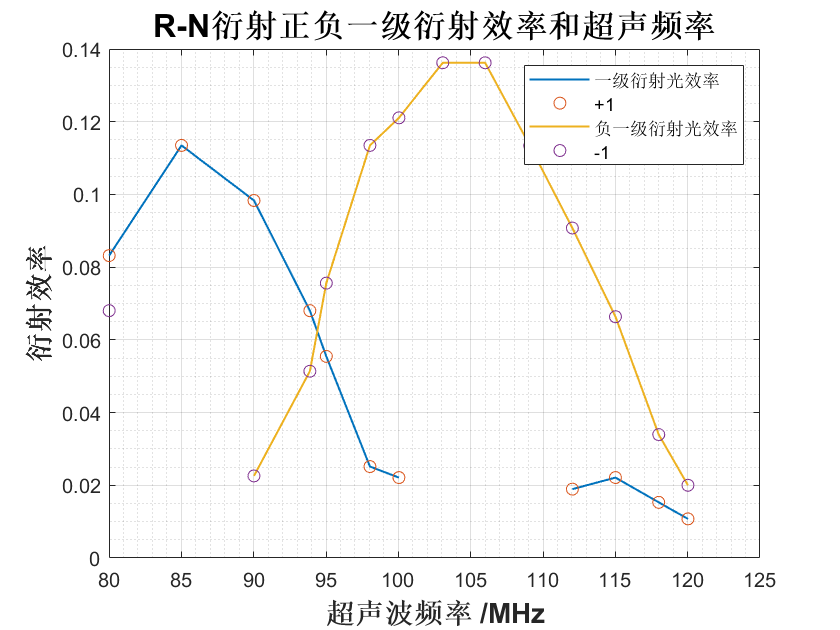
\includegraphics[width=\textwidth]{RN衍射效率随超声频率.PNG}
			\caption{Raman-Nath衍射效率与超声频率}
			\label{fig:rn_efficiency_frequency}
		\end{minipage}
		\hfill
		\begin{minipage}{0.48\textwidth}
			\centering
			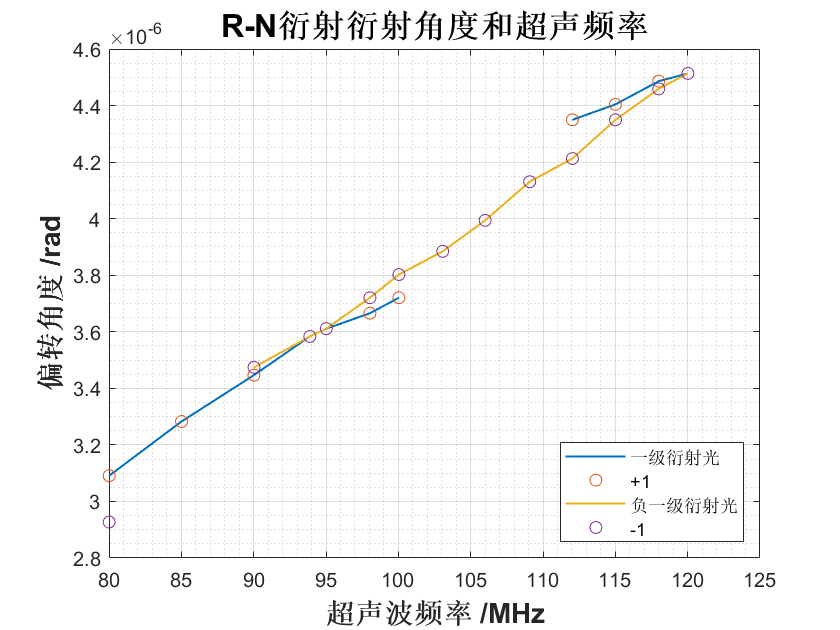
\includegraphics[width=\textwidth]{RN衍射角度随超声频率.PNG}
			\caption{Raman-Nath衍射角度与超声频率}
			\label{fig:rn_angle_frequency}
		\end{minipage}
	\end{figure}

	图中部分数据点出现了缺失，这是由于在测量过程中发现衍射光的强度较小导致难以在示波器上找到衍射峰的位置并测量其强度导致的。
	但这并不影响我们观察正负一级衍射光强度和位置与超声频率的关系。

	可以看到，正负一级衍射光效率随着超声频率的增大，二者出现相反方向的变化，呈现出此消彼长的趋势。
	而正负一级衍射光的偏转角度则随着超声频率的增大而单调增大。

\subsubsection*{6.对比Bragg衍射和Raman-Nath衍射衍射效率与电流的依赖关系}

	我们测量了Bragg衍射和Raman-Nath衍射的衍射效率与电流的依赖关系，结果如图\ref{fig:diffraction_efficiency_current}所示。

	\begin{figure}[h!]
		\centering
		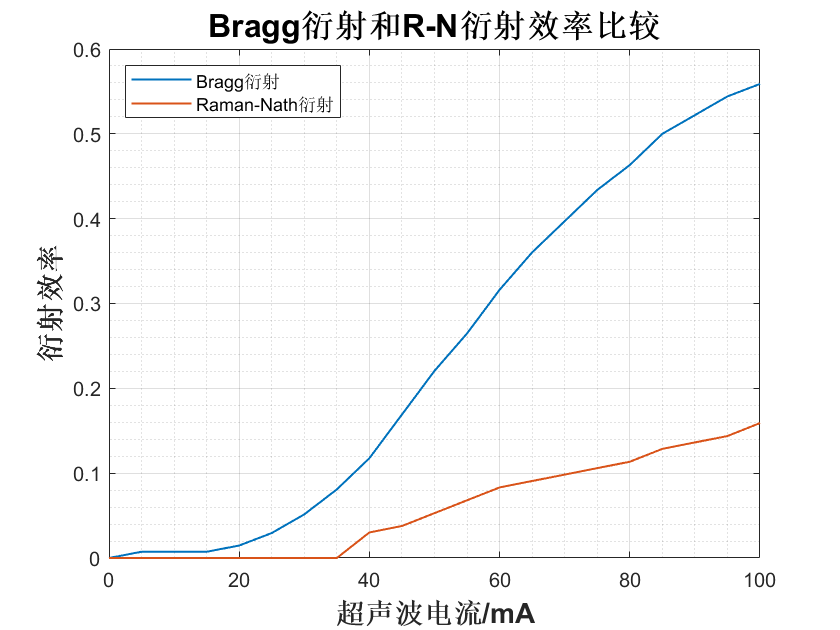
\includegraphics[width=0.8\textwidth]{衍射效率比较.png}
		\caption{两种衍射效率随电流的变化关系}
		\label{fig:diffraction_efficiency_current}
	\end{figure}

	可以看到，在不同电流的情况下，Bragg衍射的衍射效率均较高，而Raman-Nath衍射的衍射效率较低。
	这符合我们对于二者衍射效率的理论预测。

\subsubsection*{7.观察Raman-Nath衍射的二级衍射}
	我们调节晶体角度，能够观察到Raman-Nath衍射的二级衍射，如图\ref{fig:rn_second_diffraction}所示。

	\begin{figure}[h!]
		\centering
		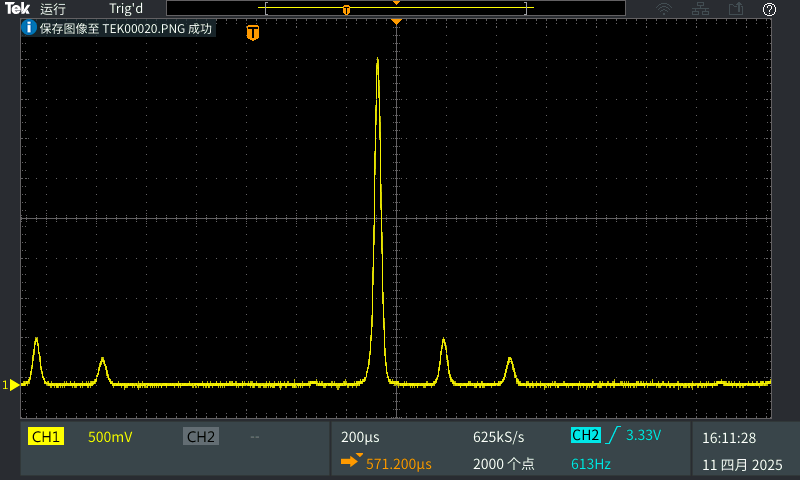
\includegraphics[width=0.8\textwidth]{TEK00021.PNG}
		\caption{Raman-Nath衍射的二级衍射}
		\label{fig:rn_second_diffraction}
	\end{figure}

	同样利用示波器测量衍射光强，可以得到零级、一级、二级衍射光的效率，如表\ref{tab:rn_second_diffraction}所示。	

	\begin{table}[h!]
		\centering
		\begin{tabular}{|c|c|c|}
			\hline
			\textbf{衍射级数} & \textbf{衍射光强 $(\mathrm{V})$} & \textbf{衍射效率} \\
			\hline
			0 & 4.05 & 0.8103 \\
			\hline
			1 & 0.599 & 0.1198 \\
			\hline
			2 & 0.349 & 0.0698 \\
			\hline
		\end{tabular}
	\end{table}

\subsubsection*{8.声光模拟通信实验}
	分别观测接收 0 级和 1 级衍射光信号时，示波器上的波形，并与发射器的波形进行对比，判断其同相还是反相。	

	我们首先测量了0级衍射光信号，如图\ref{fig:ao_communication_0}所示。

	\begin{figure}[h!]
		\centering
		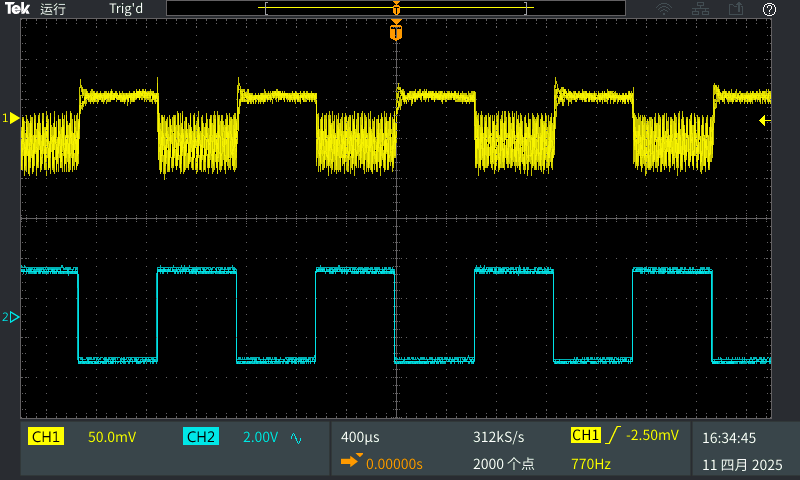
\includegraphics[width=0.8\textwidth]{TEK00023.PNG}
		\caption{0级衍射光信号}
		\label{fig:ao_communication_0}
	\end{figure}

	可以看到，0级衍射光信号与发射器的波形基本相反，说明其反相。	

	我们再测量了1级衍射光信号，如图\ref{fig:ao_communication_1}所示。

	\begin{figure}[h!]
		\centering
		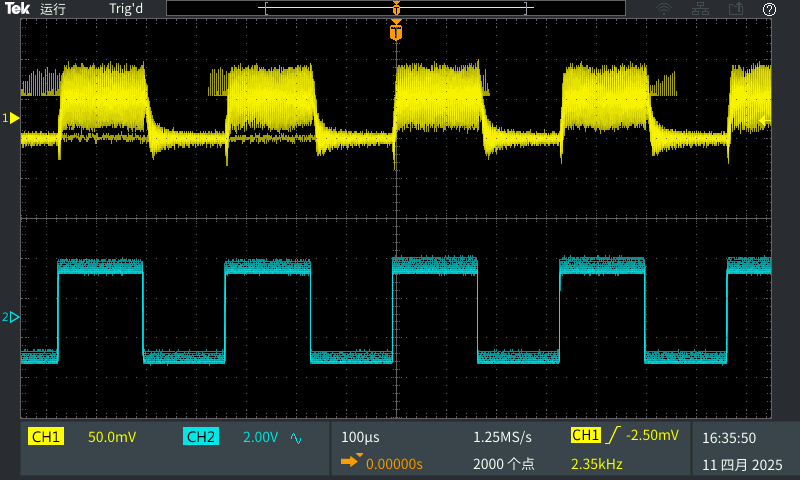
\includegraphics[width=0.8\textwidth]{TEK00024.PNG}
		\caption{1级衍射光信号}
		\label{fig:ao_communication_1}
	\end{figure}

	可以看到，1级衍射光信号与发射器的波形基本相同，说明其同相。

\subsection*{【思考题】}

\subsubsection*{1. 解释为什么Bragg衍射的效率比Raman-Nath衍射高很多？}
\textbf{答：}
Bragg衍射的高效率源于其\textbf{体光栅}特性和\textbf{动量匹配条件}的严格满足\cite{xujieping200x}：

\begin{itemize}
    \item \textbf{作用机制}：
    \begin{itemize}
        \item \textbf{Bragg衍射}：光波在较长的声光作用长度（$L \gg \Lambda^2/\lambda$）内与多个声波面相互作用，形成体光栅，能量集中到1级衍射（理论效率可达100\%）。
        \item \textbf{Raman-Nath衍射}：光波近似垂直通过薄声光栅（$L \ll \Lambda^2/\lambda$），形成多级衍射（如$\pm1$、$\pm2$级），能量分散，最高效率仅34\%（贝塞尔函数极限）。
    \end{itemize}
    
    \item \textbf{数学对比}：
    \begin{align*}
        \text{Bragg效率} &: \eta_B = \sin^2(\zeta L), \quad \text{当} \ \zeta L = \pi/2 \ \text{时} \ \eta_B = 100\% \\
        \text{Raman-Nath效率} &: \eta_R = J_1^2(2\zeta L), \quad \text{最大值仅} \ J_1^2(1.84) \approx 34\%
    \end{align*}
    
    \item \textbf{物理本质}：Bragg衍射满足动量守恒（$\vec{k}_d = \vec{k}_i \pm \vec{K}$），而Raman-Nath衍射为多级动量叠加。
\end{itemize}

\subsubsection*{2. 分别分析垂直入射时的Raman-Nath衍射与Bragg衍射中，晶体与空气界面的折射对偏转角度和声速计算的影响。}
\textbf{答：}

\begin{itemize}
    \item \textbf{Raman-Nath衍射（垂直入射）}：
    \begin{itemize}
        \item \textbf{偏转角}：衍射角$\theta_m$由$\sin \theta_m = m\lambda/\Lambda$决定，但实际测量的是空气中的角度$\phi_m$，需通过折射定律修正：
        \[
        \sin \phi_m = n \sin \theta_m = n \left( \frac{m\lambda_0}{n \Lambda} \right) = \frac{m\lambda_0}{\Lambda}
        \]
        \textbf{结论}：界面折射不影响表观偏转角（$\phi_m$直接反映$\Lambda$），但计算声速时需用介质内波长$\Lambda = v_s/f$。
        
        \item \textbf{声速计算}：直接由$v_s = \Lambda f = \frac{m\lambda_0 f}{\sin \phi_m}$得到，无需折射率修正。
    \end{itemize}
    
    \item \textbf{Bragg衍射（斜入射）}：
    \begin{itemize}
        \item \textbf{偏转角}：介质内布拉格角$\theta_B = \arcsin(\lambda/2\Lambda)$，但实测为空气中的$\phi$，需换算：
        \[
        \sin \phi = n \sin \theta_B = n \left( \frac{\lambda_0}{2n \Lambda} \right) = \frac{\lambda_0}{2\Lambda}
        \]
        \textbf{结论}：表观偏转角$\phi$仍与$\Lambda$直接相关，但计算声速时需用介质内角度$\theta_B$：
        \[
        v_s = \frac{\lambda_0 f}{2n \sin \theta_B} = \frac{\lambda_0 f}{2 \sin \phi}
        \]
        \textbf{注意}：若忽略折射率$n$，会导致声速计算值偏高。
    \end{itemize}
\end{itemize}

\subsubsection*{3. 为什么说声光器件相当于相位型光栅？}
\textbf{答：}
声光器件的本质是通过\textbf{声致折射率调制}形成周期性相位延迟，其特性如下\cite{huang200x}：

\begin{itemize}
    \item \textbf{相位调制原理}：
    超声波在介质中传播时，应变场$S(x,t)$引起折射率变化$\Delta n(x) = \frac{1}{2}n^3 P S_0 \sin(Kx-\Omega t)$，导致光波通过后的相位延迟：
    \[
    \Delta \phi(x) = k_0 \Delta n(x) L = \mu k_0 L \sin(Kx-\Omega t)
    \]
    这种周期性相位分布等效于\textbf{移动的相位光栅}。
    
    \item \textbf{与振幅光栅的区别}：
    传统振幅光栅通过吸收或反射调制光强，而声光器件仅改变光相位，无能量损失，衍射效率更高。
    
    \item \textbf{动态特性}：
    声光栅以声速$v_s$移动，导致衍射光频移（$\omega_d = \omega_i \pm \Omega$），这是振幅光栅无法实现的。
\end{itemize}

\bibliography{ref.bib} %biblatex -> 'xelatex->pdfletax->xelatex'
\bibliographystyle{ieeetr}

\subsection*{【原始数据的记录】}
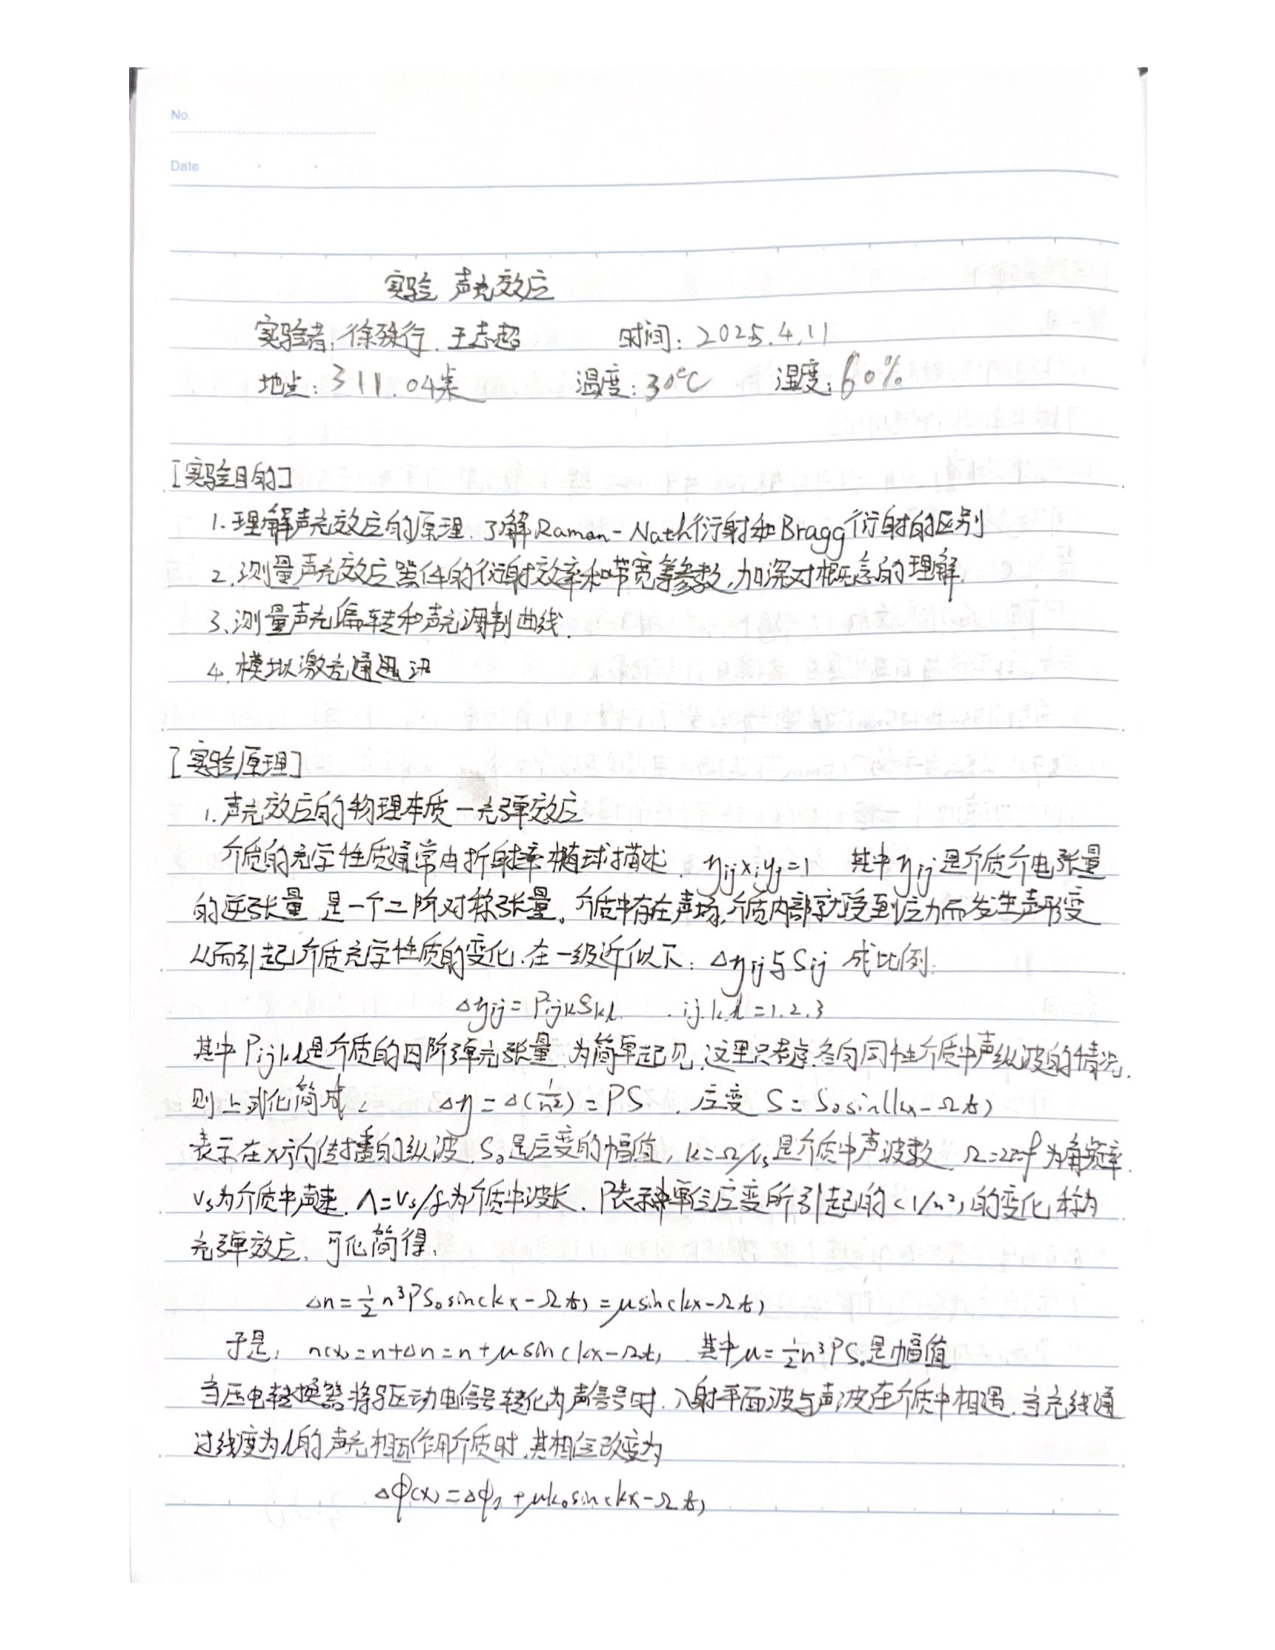
\includepdf[pages=-]{声光效应scan.pdf}

\end{document}

